\documentclass[conference]{IEEEtran}
\IEEEoverridecommandlockouts
% The preceding line is only needed to identify funding in the first footnote. If that is unneeded, please comment it out.
\usepackage{cite}
\usepackage{amsmath,amssymb,amsfonts}
\usepackage{algorithmic}
\usepackage{graphicx}
\usepackage{textcomp}
\usepackage{xcolor}
\def\BibTeX{{\rm B\kern-.05em{\sc i\kern-.025em b}\kern-.08em
    T\kern-.1667em\lower.7ex\hbox{E}\kern-.125emX}}
\begin{document}

\title{Deep Natural Language Processing Project\\Classification of Scientific Articles using SPECTER Embedding Model}

\author{\IEEEauthorblockN{Thomas Avare}
\IEEEauthorblockA{\textit{Master of Data Science, PoliTo} \\
\textit{exchange student at Politecnico di Torino from Grenbole INP - ENSIMAG}\\
Torino, Italy/Grenoble, France \\
thomas.avare@grenoble-inp.fr}}
\maketitle

\begin{abstract}
SPECTER, standing for \textit{Scientific Paper Embeddings using Citation-informed TransformERs} is a process to generate document-level embedding of scientific documents. SPECTER is based on pretrained Transformer language model and incorporating the citation graph to improve documents relatedness. SPECTER was benchmarked using SciDocs, an additional contribution to SPECTER, along previous scientific embedding models. SciDocs is an evaluation benchmark consisting of 7 document-level tasks such as citation prediction, document classification and recommendation. 

The goal of this project is to use SPECTER as a classification tool. The first part consists of understanding the principle of document-level embedding with SPECTER and its specificity, using SPECTER and SciDocs to reproduce the results presented in the original paper, focus on the text classification part being the subject of this project and some extension(s). 

In the approach of the development of SPECTER, The main idea was to use the citation-graph to introduce document relatedness into a triplet loss with  the query paper, a cited paper and a non cited paper as inputs and thus in the embedding. An idea for and extension for this project was to modify the loss to also include the date difference between the query paper and the positive paper to add/modify the information regarding the document relatedness.
\end{abstract}

\section{Introduction to SPECTER}

SPECTER (Cohan et al., 2020 \cite{b1})is an attempt to improve the embedding of sentences or whole documents by the mean of pre-trained language models to learn embeddings for scientific documents.The main idea was to incorporate inter-document relatedness into the Transformer language models such that the embedding could be more effective various tasks without any task-specific training for the embedding model. Transformer language models already exists, such as BERT, none of them used any inter-document context/information during their training. SPECTER uses the citation-graph to add inter-document context/information and these informations are used during the training of the model by the introduction of a triplet margin loss with a query paper $\mathcal P^Q$, a positive paper $\mathcal P^+$ which corresponds to a paper cited by the query paper and a negative paper $\mathcal P^-$ which corresponds to a non-cited paper by the query paper. So the triplet margin loss looks like: $$\mathcal L = \max\left\{d\left(\mathcal P^Q, \mathcal P^+\right) - d\left(\mathcal P^Q, \mathcal P^-\right) + m, 0\right\}$$ where $d$ is a distance between two embeddings, m a loss margin hyperparameter.

There are also different type of negative cases to a query paper. The "easy negatives" which are random papers not cited by the query paper and "hard negatives" which are cited paper by a cited paper but not by the query paper ($\mathcal P^1 \xrightarrow[]{cite} \mathcal P^2 \xrightarrow[]{cite}\mathcal P^3$ but $\mathcal P^1\not\xrightarrow[]{cite} \mathcal P^3$). This distinction was made provide more nuance in the training. 

They also used pretrained transformers network as a foundation for SPECTER, specifically the SciBERT (Beltagy et al., 2019\cite{b3}). After the training, it ended up becoming the state of the art model in embedding model used for various task (see next part for an introduction to SciDocs evaluation suite.

It's interesting to note that the idea of the citation graph was reused, the main idea was to transform the citation graph into a discrete space and pick the positives, easy negatives and hard negatives according to their distance in that space to the query paper and this model has become the new state of the art embedding model outperforming SPECTER (SciNCL, Ostendorff et al. 2022\cite{b2}).

\section{Introduction to Scidocs}

SciDocs (Cohan et al., 2020\cite{b1})is an evaluation framework introduce to compare different embedding models on different tasks. These tasks are Document classification, Citation prediction, user activity and Recommendation. The document classification is divided in two different type: MeSh classification, standing fro \textit{Medical Subject Headings}, and the paper topic classification known as MAG, standing for \textit{Microsoft Academic Graph}. The MeSH dataset consists of 23K academic medical papers distributed in 11 classes and the MAG consists of 25K papers distributed in 19 classes.
Since we're not interested in other tasks, we're not going to talk more about them.

\section{Goal of this Project}

The goal of this project is to use SPECTER as a tool for scientific document classification, so for MAG and MeSH classification. Another goal of this project was to introduce an extension to the initial project, I will talk about my idea in a forthcoming section, unfortunately I wasn't able to complete it but i will still briefly talk about it.

\section{The Classification Task}

As said before, SPECTER is an embedding model made to be versatile so it doesn't need any task-specific training.

\subsection{Importing SPECTER}

The first step to our classification journey was to import SPECTER. To do so, I simply cloned the official Github repository. After following the installation instructions. I had some versioning issues and one of my library wasn't downloading in the right place so I had to solve these issues. Afterwards, I was finally able to compute my first embeddings. Unfortunately, my computer doesn't have any GPU when I first started working and I decided to switch to a Google Colab notebook to pursue my experiments.

Before training my first models, I imported the SPECTER model accessible through the huggingFace transformer's library, then I imported the data provided by SiDocs. This contains all the data used for the SciDocs benchmarking, including the information of all papers (paper id, author, title, abstract, date of publication, citations and cited by), their classification (MAG and MeSH) and their embeddings. To import and manage all these informations, I used Pandas DataFrames which is really easy and convenient for these kind of tasks.

\subsection{Importing the Data}

After my first experiments to train models, I realized that it was not working for a very simple reason. The embeddings provided with SciDocs are those computed with the SPECTER model from the SPECTER GitHub and the SPECTER model from the HuggingFace Transformer library computes different embeddings for the same title and abstract. So I re-computed the embeddings used for the MAG and MeSH classifications and saved it inn a json file, for every paper, we have the paper id, The paper id, the title, the abstract and its embedding. To prepare the data for the classification, we simply have to import these information into a data frame and import the classification and merge it according to their paper id. The classification is already split into a train/test dataset for reproducibility purposes for the SciDocs benchmarking.

\subsection{Training Models}

After correctly importing the data and solving our embedding issues. Now we can train models for our classification task. I trained multiple types of models and will compare their performances according to their f1 score on the test dataset. Unfortunately, even by mimicking the training routine used for the SciDocs, I was never able to level or top it.

\texttt{Here a table with the results for MAG first and will do MeSH later}

Explaining how I trained the models with a gridsearch for parameters and another part for CNN. 


\subsection{Units}
\begin{itemize}
\item Use either SI (MKS) or CGS as primary units. (SI units are encouraged.) English units may be used as secondary units (in parentheses). An exception would be the use of English units as identifiers in trade, such as ``3.5-inch disk drive''.
\item Avoid combining SI and CGS units, such as current in amperes and magnetic field in oersteds. This often leads to confusion because equations do not balance dimensionally. If you must use mixed units, clearly state the units for each quantity that you use in an equation.
\item Do not mix complete spellings and abbreviations of units: ``Wb/m\textsuperscript{2}'' or ``webers per square meter'', not ``webers/m\textsuperscript{2}''. Spell out units when they appear in text: ``. . . a few henries'', not ``. . . a few H''.
\item Use a zero before decimal points: ``0.25'', not ``.25''. Use ``cm\textsuperscript{3}'', not ``cc''.)
\end{itemize}

\subsection{Equations}
Number equations consecutively. To make your 
equations more compact, you may use the solidus (~/~), the exp function, or 
appropriate exponents. Italicize Roman symbols for quantities and variables, 
but not Greek symbols. Use a long dash rather than a hyphen for a minus 
sign. Punctuate equations with commas or periods when they are part of a 
sentence, as in:
\begin{equation}
a+b=\gamma\label{eq}
\end{equation}

Be sure that the 
symbols in your equation have been defined before or immediately following 
the equation. Use ``\eqref{eq}'', not ``Eq.~\eqref{eq}'' or ``equation \eqref{eq}'', except at 
the beginning of a sentence: ``Equation \eqref{eq} is . . .''

\subsection{\LaTeX-Specific Advice}

Please use ``soft'' (e.g., \verb|\eqref{Eq}|) cross references instead
of ``hard'' references (e.g., \verb|(1)|). That will make it possible
to combine sections, add equations, or change the order of figures or
citations without having to go through the file line by line.

Please don't use the \verb|{eqnarray}| equation environment. Use
\verb|{align}| or \verb|{IEEEeqnarray}| instead. The \verb|{eqnarray}|
environment leaves unsightly spaces around relation symbols.

Please note that the \verb|{subequations}| environment in {\LaTeX}
will increment the main equation counter even when there are no
equation numbers displayed. If you forget that, you might write an
article in which the equation numbers skip from (17) to (20), causing
the copy editors to wonder if you've discovered a new method of
counting.

{\BibTeX} does not work by magic. It doesn't get the bibliographic
data from thin air but from .bib files. If you use {\BibTeX} to produce a
bibliography you must send the .bib files. 

{\LaTeX} can't read your mind. If you assign the same label to a
subsubsection and a table, you might find that Table I has been cross
referenced as Table IV-B3. 

{\LaTeX} does not have precognitive abilities. If you put a
\verb|\label| command before the command that updates the counter it's
supposed to be using, the label will pick up the last counter to be
cross referenced instead. In particular, a \verb|\label| command
should not go before the caption of a figure or a table.

Do not use \verb|\nonumber| inside the \verb|{array}| environment. It
will not stop equation numbers inside \verb|{array}| (there won't be
any anyway) and it might stop a wanted equation number in the
surrounding equation.

\subsection{Some Common Mistakes}\label{SCM}
\begin{itemize}
\item The word ``data'' is plural, not singular.
\item The subscript for the permeability of vacuum $\mu_{0}$, and other common scientific constants, is zero with subscript formatting, not a lowercase letter ``o''.
\item In American English, commas, semicolons, periods, question and exclamation marks are located within quotation marks only when a complete thought or name is cited, such as a title or full quotation. When quotation marks are used, instead of a bold or italic typeface, to highlight a word or phrase, punctuation should appear outside of the quotation marks. A parenthetical phrase or statement at the end of a sentence is punctuated outside of the closing parenthesis (like this). (A parenthetical sentence is punctuated within the parentheses.)
\item A graph within a graph is an ``inset'', not an ``insert''. The word alternatively is preferred to the word ``alternately'' (unless you really mean something that alternates).
\item Do not use the word ``essentially'' to mean ``approximately'' or ``effectively''.
\item In your paper title, if the words ``that uses'' can accurately replace the word ``using'', capitalize the ``u''; if not, keep using lower-cased.
\item Be aware of the different meanings of the homophones ``affect'' and ``effect'', ``complement'' and ``compliment'', ``discreet'' and ``discrete'', ``principal'' and ``principle''.
\item Do not confuse ``imply'' and ``infer''.
\item The prefix ``non'' is not a word; it should be joined to the word it modifies, usually without a hyphen.
\item There is no period after the ``et'' in the Latin abbreviation ``et al.''.
\item The abbreviation ``i.e.'' means ``that is'', and the abbreviation ``e.g.'' means ``for example''.
\end{itemize}
An excellent style manual for science writers is \cite{b7}.

\subsection{Authors and Affiliations}
\textbf{The class file is designed for, but not limited to, six authors.} A 
minimum of one author is required for all conference articles. Author names 
should be listed starting from left to right and then moving down to the 
next line. This is the author sequence that will be used in future citations 
and by indexing services. Names should not be listed in columns nor group by 
affiliation. Please keep your affiliations as succinct as possible (for 
example, do not differentiate among departments of the same organization).

\subsection{Identify the Headings}
Headings, or heads, are organizational devices that guide the reader through 
your paper. There are two types: component heads and text heads.

Component heads identify the different components of your paper and are not 
topically subordinate to each other. Examples include Acknowledgments and 
References and, for these, the correct style to use is ``Heading 5''. Use 
``figure caption'' for your Figure captions, and ``table head'' for your 
table title. Run-in heads, such as ``Abstract'', will require you to apply a 
style (in this case, italic) in addition to the style provided by the drop 
down menu to differentiate the head from the text.

Text heads organize the topics on a relational, hierarchical basis. For 
example, the paper title is the primary text head because all subsequent 
material relates and elaborates on this one topic. If there are two or more 
sub-topics, the next level head (uppercase Roman numerals) should be used 
and, conversely, if there are not at least two sub-topics, then no subheads 
should be introduced.

\subsection{Figures and Tables}
\paragraph{Positioning Figures and Tables} Place figures and tables at the top and 
bottom of columns. Avoid placing them in the middle of columns. Large 
figures and tables may span across both columns. Figure captions should be 
below the figures; table heads should appear above the tables. Insert 
figures and tables after they are cited in the text. Use the abbreviation 
``Fig.~\ref{fig}'', even at the beginning of a sentence.

\begin{table}[htbp]
\caption{Table Type Styles}
\begin{center}
\begin{tabular}{|c|c|c|c|}
\hline
\textbf{Table}&\multicolumn{3}{|c|}{\textbf{Table Column Head}} \\
\cline{2-4} 
\textbf{Head} & \textbf{\textit{Table column subhead}}& \textbf{\textit{Subhead}}& \textbf{\textit{Subhead}} \\
\hline
copy& More table copy$^{\mathrm{a}}$& &  \\
\hline
\multicolumn{4}{l}{$^{\mathrm{a}}$Sample of a Table footnote.}
\end{tabular}
\label{tab1}
\end{center}
\end{table}

\begin{figure}[htbp]
\centerline{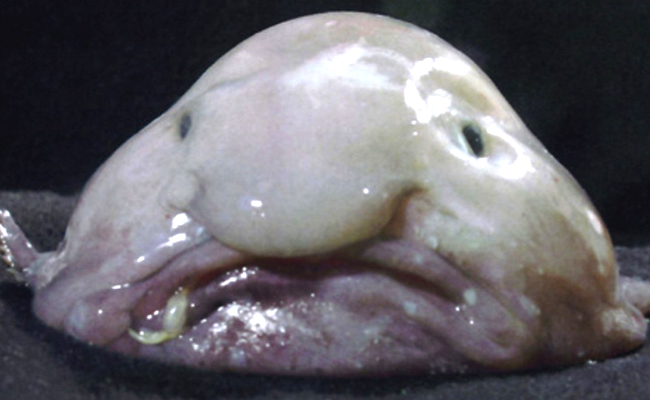
\includegraphics[width=0.4\textwidth]{fig1}}
\caption{Example of a figure caption.}
\label{fig}
\end{figure}

Figure Labels: Use 8 point Times New Roman for Figure labels. Use words 
rather than symbols or abbreviations when writing Figure axis labels to 
avoid confusing the reader. As an example, write the quantity 
``Magnetization'', or ``Magnetization, M'', not just ``M''. If including 
units in the label, present them within parentheses. Do not label axes only 
with units. In the example, write ``Magnetization (A/m)'' or ``Magnetization 
\{A[m(1)]\}'', not just ``A/m''. Do not label axes with a ratio of 
quantities and units. For example, write ``Temperature (K)'', not 
``Temperature/K''.

\section*{Acknowledgment}

The preferred spelling of the word ``acknowledgment'' in America is without 
an ``e'' after the ``g''. Avoid the stilted expression ``one of us (R. B. 
G.) thanks $\ldots$''. Instead, try ``R. B. G. thanks$\ldots$''. Put sponsor 
acknowledgments in the unnumbered footnote on the first page.

\section*{References}

Please number citations consecutively within brackets . The 
sentence punctuation follows the bracket \cite{b2}. Refer simply to the reference 
number, as in \cite{b3}---do not use ``Ref. \cite{b3}'' or ``reference \cite{b3}'' except at 
the beginning of a sentence: ``Reference \cite{b3} was the first $\ldots$''

Number footnotes separately in superscripts. Place the actual footnote at 
the bottom of the column in which it was cited. Do not put footnotes in the 
abstract or reference list. Use letters for table footnotes.

Unless there are six authors or more give all authors' names; do not use 
``et al.''. Papers that have not been published, even if they have been 
submitted for publication, should be cited as ``unpublished'' \cite{b4}. Papers 
that have been accepted for publication should be cited as ``in press'' \cite{b5}. 
Capitalize only the first word in a paper title, except for proper nouns and 
element symbols.

For papers published in translation journals, please give the English 
citation first, followed by the original foreign-language citation \cite{b6}.

\begin{thebibliography}{00}
\bibitem{b1}Arman Cohan, Sergey Feldman, Iz Beltagy, Doug Downey, and Daniel Weld. 

2020. SPECTER: Document-level Representation Learning using Citation-informed Transformers

\bibitem{b2} Malte Ostendorff, Nils Rethmeier, Isabelle Augenstein, Bela Gipp, Georg Rehm.

2022. Neighborhood Contrastive Learning for Scientific Document Representations with Citation Embeddings
\bibitem{b3} Iz Beltagy, Kyle Lo, and Arman Cohan.

2019. SciB- ERT: A Pretrained Language Model for Scientific Text. In EMNLP.

\end{thebibliography}
\vspace{12pt}

\end{document}

